
%%%%%%%%%%%%%%%%%%%%%%%%%%%%%%%%%%%%%%%%%%%%%%%%%%%%%%%%%%%%%%%
%
% Welcome to Overleaf --- just edit your LaTeX on the left,
% and we'll compile it for you on the right. If you open the
% 'Share' menu, you can invite other users to edit at the same
% time. See www.overleaf.com/learn for more info. Enjoy!
%
%%%%%%%%%%%%%%%%%%%%%%%%%%%%%%%%%%%%%%%%%%%%%%%%%%%%%%%%%%%%%%%
\documentclass{exam}

\usepackage{graphicx}
\graphicspath{ {./images/} }

\lhead{ECON 2010}
\chead{Practice}
\lfoot{10/26/2022}
\rhead{Fall 2022}

% \printanswers
\noprintanswers

\begin{document}

\section{Practice Questions}

\begin{questions}
\question (Exam 2 - 2019Q2) Antitrust authorities in several countries brought legal action against an international cartel that produced Cathode Ray Tubes (“CRTs”). CRTs are the prior generation of television screens and computer monitors before the introduction and adoption
of High Definition Television (“HDTV”). In its day, the CRT cartel was considered to be effective in “fixing” the market price and output
\begin{parts}
\part According to the economic theory of cartles, what is the likely effect on the price and the market quantity of CRTs once the CRT cartel is up and running?
\begin{solution} Once the cartel is up and running it will want to act as a single monopolist firm, colluding on the monopolist price and quantity of CRTs. This will \textbf{reduce} the market quantity of CRTs and \textbf{increase} the price of CRTs. \end{solution}
\part What is the likely effect of the CRT cartel upon the price of television sets that have CRT screens? 
\begin{solution} The CRT cartel will increase the price of CRTs, which are a crucial input for CRT screen televisions. The increased cost of an input will cause the supply curve of televisions to shift up, resulting in an \textbf{increase} in the price of televisions. \end{solution}
\part IAN CRT is the name of the one CRT producer that did not join the CRT cartel. What is the likely economic consequence of the cartel for this firm?
\begin{solution} IAN CRT will be able to sell CRTs at the monopoly price without restricting its quantity. As a result, its profits will be \textbf{higher} than the colluding firms (assuming comparable costs). \end{solution}
\part The economic theory of cartels reveals a temptation that exists for each member of a functioning cartel. Identify and explain what it is.
\begin{solution} The temptation for each member of a functioning cartel is to defect from (or “cheat on”) the agreed upon production quantity. Any firm that defects from the cartel can increase its output. This will lead to higher profits for the defecting firms. \end{solution}
\part What is the likely effect of a CRT cartel upon the introduction of new screen technology (such as HDTV screens)?
\begin{solution} The CRT cartel may speed up the introduction of new screen technology because entrepreneurs can introduce a new technology at a higher price than they would be able to in a competitive market for television screens. The cartel
creates an additional incentive for innovation. \end{solution}
\part Under U.S. antitrust law, is participating in a price-fixing cartel illegal, legal, or one cannot say because “it all depends”?
\begin{solution} It is illegal to participate in a price-fixing cartel. It is legal to implicitly coordinate prices, as long as there is no explicit agreement to do so. \end{solution}
\end{parts}

\question (Exam 2 - 2019Q5) Keeley is a Vice-President of Sales for a major consumer goods company and she tells her staff, “We are fortunate; there are very few substitutes for our product; demand is inelastic. Unlike firms that face a lot of competition, we have lots of discretion in setting our prices.” Raed, a junior member of her staff responds, “But wouldn’t we want to set our price in the elastic portion of the demand curve?” Use your knowledge of economic theory to clarify what is being said here.
\begin{solution} Keeley claims that the firm is a price-maker. Rather than taking the market price as given, the firm has chosen a price in the inelastic part of the demand curve. 

Raed observes that inelastic demand implies that the firm could increase revenue by increasing its price. An increase in $P$ will have a negligable effect on $Q$, resulting in higher revenues.  A firm with market power will always set a price somewhere in the elastic part of the demand curve. \end{solution}

\question (Exam 2 - 2022Q2) The business firm shown below makes buttons, an important product for consumers of blouses, shirts, and coats.  It is the only button firm in Centralia, a planned economy whose Constitution states the all manufacturing firms are to be operated in the best interests of consumers.

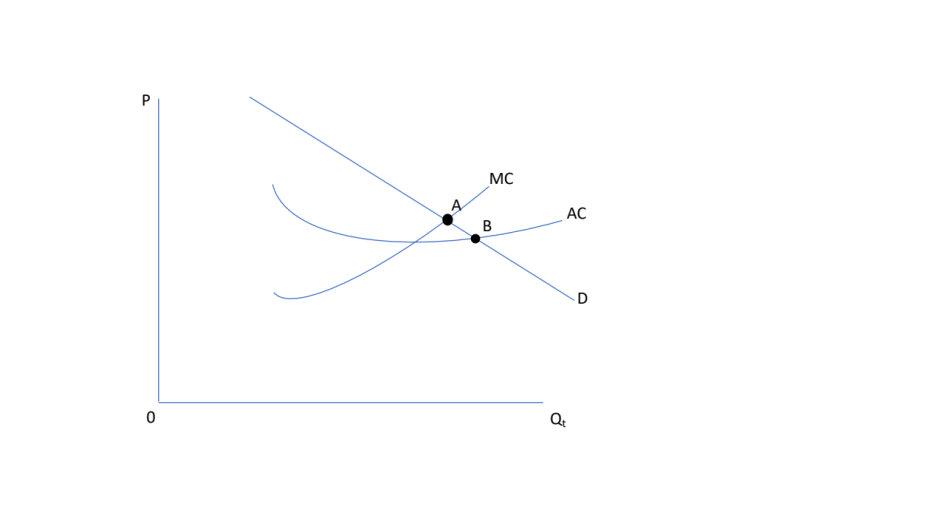
\includegraphics[width = \textwidth]{E2-2020Q2.png}

\begin{parts} 
\part Your supervisor asks you whether the button factory should operate at the price-quantity combination shown as point $A$.  What do you tell your supervisor and why?
\begin{solution} We should produce at point $A$. At this point, the marginal social benefit of an additional button (measured by the $D$ curve) is equal to the marginal cost of production (measured by the $MC$ curve). \end{solution}
\part Your supervisor asks, “But what about the price-quantity combination at point $B$?”  What do you tell your supervisor, and why?
\begin{solution} We should \textbf{not} produce at $B$. At this quantity, the marginal cost of the last button we produce is \textbf{higher} than anyone is willing to pay.\end{solution}
\part Assume Centralia gets a new Constitution and this button factory no longer must operate in the best interests of consumers.  Indeed, your supervisor now owns the button factory and wants to maximize the firm’s profits.  Your supervisor turns to you for advice and asks, “What price and output should I select to maximize profits (or minimize losses)”?  What’s the correct answer, and why? \begin{solution} The button factory should price at the point where $MR = MC$.

Because the button factory is a monopolist, its $MR$ curve will be inside of and steeper than the demand curve. The resulting price will be \textbf{higher} and the quantity \textbf{lower} than that chosen in part (a). \end{solution}
\end{parts}

\end{questions}


\end{document}
